\documentclass[twoside]{book}

% Packages required by doxygen
\usepackage{fixltx2e}
\usepackage{calc}
\usepackage{doxygen}
\usepackage[export]{adjustbox} % also loads graphicx
\usepackage{graphicx}
\usepackage[utf8]{inputenc}
\usepackage{makeidx}
\usepackage{multicol}
\usepackage{multirow}
\PassOptionsToPackage{warn}{textcomp}
\usepackage{textcomp}
\usepackage[nointegrals]{wasysym}
\usepackage[table]{xcolor}

% Font selection
\usepackage[T1]{fontenc}
\usepackage[scaled=.90]{helvet}
\usepackage{courier}
\usepackage{amssymb}
\usepackage{sectsty}
\renewcommand{\familydefault}{\sfdefault}
\allsectionsfont{%
  \fontseries{bc}\selectfont%
  \color{darkgray}%
}
\renewcommand{\DoxyLabelFont}{%
  \fontseries{bc}\selectfont%
  \color{darkgray}%
}
\newcommand{\+}{\discretionary{\mbox{\scriptsize$\hookleftarrow$}}{}{}}

% Page & text layout
\usepackage{geometry}
\geometry{%
  a4paper,%
  top=2.5cm,%
  bottom=2.5cm,%
  left=2.5cm,%
  right=2.5cm%
}
\tolerance=750
\hfuzz=15pt
\hbadness=750
\setlength{\emergencystretch}{15pt}
\setlength{\parindent}{0cm}
\setlength{\parskip}{3ex plus 2ex minus 2ex}
\makeatletter
\renewcommand{\paragraph}{%
  \@startsection{paragraph}{4}{0ex}{-1.0ex}{1.0ex}{%
    \normalfont\normalsize\bfseries\SS@parafont%
  }%
}
\renewcommand{\subparagraph}{%
  \@startsection{subparagraph}{5}{0ex}{-1.0ex}{1.0ex}{%
    \normalfont\normalsize\bfseries\SS@subparafont%
  }%
}
\makeatother

% Headers & footers
\usepackage{fancyhdr}
\pagestyle{fancyplain}
\fancyhead[LE]{\fancyplain{}{\bfseries\thepage}}
\fancyhead[CE]{\fancyplain{}{}}
\fancyhead[RE]{\fancyplain{}{\bfseries\leftmark}}
\fancyhead[LO]{\fancyplain{}{\bfseries\rightmark}}
\fancyhead[CO]{\fancyplain{}{}}
\fancyhead[RO]{\fancyplain{}{\bfseries\thepage}}
\fancyfoot[LE]{\fancyplain{}{}}
\fancyfoot[CE]{\fancyplain{}{}}
\fancyfoot[RE]{\fancyplain{}{\bfseries\scriptsize Generated by Doxygen }}
\fancyfoot[LO]{\fancyplain{}{\bfseries\scriptsize Generated by Doxygen }}
\fancyfoot[CO]{\fancyplain{}{}}
\fancyfoot[RO]{\fancyplain{}{}}
\renewcommand{\footrulewidth}{0.4pt}
\renewcommand{\chaptermark}[1]{%
  \markboth{#1}{}%
}
\renewcommand{\sectionmark}[1]{%
  \markright{\thesection\ #1}%
}

% Indices & bibliography
\usepackage{natbib}
\usepackage[titles]{tocloft}
\setcounter{tocdepth}{3}
\setcounter{secnumdepth}{5}
\makeindex

% Hyperlinks (required, but should be loaded last)
\usepackage{ifpdf}
\ifpdf
  \usepackage[pdftex,pagebackref=true]{hyperref}
\else
  \usepackage[ps2pdf,pagebackref=true]{hyperref}
\fi
\hypersetup{%
  colorlinks=true,%
  linkcolor=blue,%
  citecolor=blue,%
  unicode%
}

% Custom commands
\newcommand{\clearemptydoublepage}{%
  \newpage{\pagestyle{empty}\cleardoublepage}%
}

\usepackage{caption}
\captionsetup{labelsep=space,justification=centering,font={bf},singlelinecheck=off,skip=4pt,position=top}

%===== C O N T E N T S =====

\begin{document}

% Titlepage & ToC
\hypersetup{pageanchor=false,
             bookmarksnumbered=true,
             pdfencoding=unicode
            }
\pagenumbering{alph}
\begin{titlepage}
\vspace*{7cm}
\begin{center}%
{\Large Service de gestion de clôtures des fiches de frais }\\
\vspace*{1cm}
{\large Generated by Doxygen 1.8.14}\\
\end{center}
\end{titlepage}
\clearemptydoublepage
\pagenumbering{roman}
\tableofcontents
\clearemptydoublepage
\pagenumbering{arabic}
\hypersetup{pageanchor=true}

%--- Begin generated contents ---
\chapter{Namespace Index}
\section{Packages}
Here are the packages with brief descriptions (if available)\+:\begin{DoxyCompactList}
\item\contentsline{section}{\mbox{\hyperlink{namespacebibliotheque_classes}{bibliotheque\+Classes}} }{\pageref{namespacebibliotheque_classes}}{}
\item\contentsline{section}{\mbox{\hyperlink{namespacegestion_cloture}{gestion\+Cloture}} }{\pageref{namespacegestion_cloture}}{}
\item\contentsline{section}{\mbox{\hyperlink{namespacegestion_cloture_1_1_tests}{gestion\+Cloture.\+Tests}} }{\pageref{namespacegestion_cloture_1_1_tests}}{}
\item\contentsline{section}{\mbox{\hyperlink{namespace_windows_service2}{Windows\+Service2}} }{\pageref{namespace_windows_service2}}{}
\end{DoxyCompactList}

\chapter{Hierarchical Index}
\section{Class Hierarchy}
This inheritance list is sorted roughly, but not completely, alphabetically\+:\begin{DoxyCompactList}
\item \contentsline{section}{bibliotheque\+Classes.\+acces\+Donnees}{\pageref{classbibliotheque_classes_1_1acces_donnees}}{}
\item \contentsline{section}{gestion\+Cloture.\+Tests.\+Form2\+Tests}{\pageref{classgestion_cloture_1_1_tests_1_1_form2_tests}}{}
\item \contentsline{section}{gestion\+Cloture.\+gestion\+Date}{\pageref{classgestion_cloture_1_1gestion_date}}{}
\item \contentsline{section}{Windows\+Service2.\+Program}{\pageref{class_windows_service2_1_1_program}}{}
\item Service\+Base\begin{DoxyCompactList}
\item \contentsline{section}{Windows\+Service2.\+Service1}{\pageref{class_windows_service2_1_1_service1}}{}
\end{DoxyCompactList}
\end{DoxyCompactList}

\chapter{Class Index}
\section{Class List}
Here are the classes, structs, unions and interfaces with brief descriptions\+:\begin{DoxyCompactList}
\item\contentsline{section}{\mbox{\hyperlink{classbibliotheque_classes_1_1acces_donnees}{bibliotheque\+Classes.\+acces\+Donnees}} \\*Classe d\textquotesingle{}accès aux données }{\pageref{classbibliotheque_classes_1_1acces_donnees}}{}
\item\contentsline{section}{\mbox{\hyperlink{classgestion_cloture_1_1_tests_1_1_form2_tests}{gestion\+Cloture.\+Tests.\+Form2\+Tests}} }{\pageref{classgestion_cloture_1_1_tests_1_1_form2_tests}}{}
\item\contentsline{section}{\mbox{\hyperlink{classgestion_cloture_1_1gestion_date}{gestion\+Cloture.\+gestion\+Date}} \\*Classe de gestion des dates }{\pageref{classgestion_cloture_1_1gestion_date}}{}
\item\contentsline{section}{\mbox{\hyperlink{class_windows_service2_1_1_program}{Windows\+Service2.\+Program}} }{\pageref{class_windows_service2_1_1_program}}{}
\item\contentsline{section}{\mbox{\hyperlink{class_windows_service2_1_1_service1}{Windows\+Service2.\+Service1}} }{\pageref{class_windows_service2_1_1_service1}}{}
\end{DoxyCompactList}

\chapter{Namespace Documentation}
\hypertarget{namespacebibliotheque_classes}{}\section{bibliotheque\+Classes Namespace Reference}
\label{namespacebibliotheque_classes}\index{bibliotheque\+Classes@{bibliotheque\+Classes}}
\subsection*{Classes}
\begin{DoxyCompactItemize}
\item 
class \mbox{\hyperlink{classbibliotheque_classes_1_1acces_donnees}{acces\+Donnees}}
\begin{DoxyCompactList}\small\item\em Classe d\textquotesingle{}accès aux données \end{DoxyCompactList}\end{DoxyCompactItemize}

\hypertarget{namespacegestion_cloture}{}\section{gestion\+Cloture Namespace Reference}
\label{namespacegestion_cloture}\index{gestion\+Cloture@{gestion\+Cloture}}
\subsection*{Namespaces}
\begin{DoxyCompactItemize}
\end{DoxyCompactItemize}
\subsection*{Classes}
\begin{DoxyCompactItemize}
\item 
class \mbox{\hyperlink{classgestion_cloture_1_1gestion_date}{gestion\+Date}}
\begin{DoxyCompactList}\small\item\em Classe de gestion des dates \end{DoxyCompactList}\end{DoxyCompactItemize}

\hypertarget{namespacegestion_cloture_1_1_tests}{}\section{gestion\+Cloture.\+Tests Namespace Reference}
\label{namespacegestion_cloture_1_1_tests}\index{gestion\+Cloture.\+Tests@{gestion\+Cloture.\+Tests}}
\subsection*{Classes}
\begin{DoxyCompactItemize}
\item 
class \mbox{\hyperlink{classgestion_cloture_1_1_tests_1_1_form2_tests}{Form2\+Tests}}
\end{DoxyCompactItemize}

\hypertarget{namespace_windows_service2}{}\section{Windows\+Service2 Namespace Reference}
\label{namespace_windows_service2}\index{Windows\+Service2@{Windows\+Service2}}
\subsection*{Classes}
\begin{DoxyCompactItemize}
\item 
class \mbox{\hyperlink{class_windows_service2_1_1_program}{Program}}
\item 
class \mbox{\hyperlink{class_windows_service2_1_1_service1}{Service1}}
\end{DoxyCompactItemize}

\chapter{Class Documentation}
\hypertarget{classbibliotheque_classes_1_1acces_donnees}{}\section{bibliotheque\+Classes.\+acces\+Donnees Class Reference}
\label{classbibliotheque_classes_1_1acces_donnees}\index{bibliotheque\+Classes.\+acces\+Donnees@{bibliotheque\+Classes.\+acces\+Donnees}}


Classe d\textquotesingle{}accès aux données  


\subsection*{Public Member Functions}
\begin{DoxyCompactItemize}
\item 
void \mbox{\hyperlink{classbibliotheque_classes_1_1acces_donnees_a3d5707c0c32ffef3ffb96024c429962c}{selection\+Fiche}} ()
\begin{DoxyCompactList}\small\item\em Cette méthode permet de sélectionner toutes les fiches de frais et de les écrire dans un fichier de sortie présent dans le répertoire de l\textquotesingle{}application \end{DoxyCompactList}\item 
void \mbox{\hyperlink{classbibliotheque_classes_1_1acces_donnees_a28c549fe1997665d275fd37d97414990}{selection\+Fiche\+Mois\+Precedent}} ()
\begin{DoxyCompactList}\small\item\em Cette méthode permet de sélectionner les fiches de frais du mois précédent et de les écrire dans un fichier de sortie présent dans le répertoire de l\textquotesingle{}application \end{DoxyCompactList}\item 
void \mbox{\hyperlink{classbibliotheque_classes_1_1acces_donnees_a05d611d9c6a77bdcf589092a68e6d262}{mise\+A\+Jour\+Fiche\+Validation}} ()
\begin{DoxyCompactList}\small\item\em Cette méthode permet de mettre à jour les fiches de frais du mois précédent en les mettant à l\textquotesingle{}état \char`\"{}\+C\+L\char`\"{} (clôturée) \end{DoxyCompactList}\item 
void \mbox{\hyperlink{classbibliotheque_classes_1_1acces_donnees_a3f6ab640fe018b0143515d0d8cbeda80}{mise\+A\+Jour\+Fiche\+Remboursement}} ()
\begin{DoxyCompactList}\small\item\em Cette méthode permet de mettre à jour les fiches de frais validées et du mois précédent en les mettant à l\textquotesingle{}état \char`\"{}\+R\+B\char`\"{} (remboursé) \end{DoxyCompactList}\end{DoxyCompactItemize}


\subsection{Detailed Description}
Classe d\textquotesingle{}accès aux données 



\subsection{Member Function Documentation}
\mbox{\Hypertarget{classbibliotheque_classes_1_1acces_donnees_a3f6ab640fe018b0143515d0d8cbeda80}\label{classbibliotheque_classes_1_1acces_donnees_a3f6ab640fe018b0143515d0d8cbeda80}} 
\index{bibliotheque\+Classes\+::acces\+Donnees@{bibliotheque\+Classes\+::acces\+Donnees}!mise\+A\+Jour\+Fiche\+Remboursement@{mise\+A\+Jour\+Fiche\+Remboursement}}
\index{mise\+A\+Jour\+Fiche\+Remboursement@{mise\+A\+Jour\+Fiche\+Remboursement}!bibliotheque\+Classes\+::acces\+Donnees@{bibliotheque\+Classes\+::acces\+Donnees}}
\subsubsection{\texorpdfstring{mise\+A\+Jour\+Fiche\+Remboursement()}{miseAJourFicheRemboursement()}}
{\footnotesize\ttfamily void bibliotheque\+Classes.\+acces\+Donnees.\+mise\+A\+Jour\+Fiche\+Remboursement (\begin{DoxyParamCaption}{ }\end{DoxyParamCaption})}



Cette méthode permet de mettre à jour les fiches de frais validées et du mois précédent en les mettant à l\textquotesingle{}état \char`\"{}\+R\+B\char`\"{} (remboursé) 

\mbox{\Hypertarget{classbibliotheque_classes_1_1acces_donnees_a05d611d9c6a77bdcf589092a68e6d262}\label{classbibliotheque_classes_1_1acces_donnees_a05d611d9c6a77bdcf589092a68e6d262}} 
\index{bibliotheque\+Classes\+::acces\+Donnees@{bibliotheque\+Classes\+::acces\+Donnees}!mise\+A\+Jour\+Fiche\+Validation@{mise\+A\+Jour\+Fiche\+Validation}}
\index{mise\+A\+Jour\+Fiche\+Validation@{mise\+A\+Jour\+Fiche\+Validation}!bibliotheque\+Classes\+::acces\+Donnees@{bibliotheque\+Classes\+::acces\+Donnees}}
\subsubsection{\texorpdfstring{mise\+A\+Jour\+Fiche\+Validation()}{miseAJourFicheValidation()}}
{\footnotesize\ttfamily void bibliotheque\+Classes.\+acces\+Donnees.\+mise\+A\+Jour\+Fiche\+Validation (\begin{DoxyParamCaption}{ }\end{DoxyParamCaption})}



Cette méthode permet de mettre à jour les fiches de frais du mois précédent en les mettant à l\textquotesingle{}état \char`\"{}\+C\+L\char`\"{} (clôturée) 

\mbox{\Hypertarget{classbibliotheque_classes_1_1acces_donnees_a3d5707c0c32ffef3ffb96024c429962c}\label{classbibliotheque_classes_1_1acces_donnees_a3d5707c0c32ffef3ffb96024c429962c}} 
\index{bibliotheque\+Classes\+::acces\+Donnees@{bibliotheque\+Classes\+::acces\+Donnees}!selection\+Fiche@{selection\+Fiche}}
\index{selection\+Fiche@{selection\+Fiche}!bibliotheque\+Classes\+::acces\+Donnees@{bibliotheque\+Classes\+::acces\+Donnees}}
\subsubsection{\texorpdfstring{selection\+Fiche()}{selectionFiche()}}
{\footnotesize\ttfamily void bibliotheque\+Classes.\+acces\+Donnees.\+selection\+Fiche (\begin{DoxyParamCaption}{ }\end{DoxyParamCaption})}



Cette méthode permet de sélectionner toutes les fiches de frais et de les écrire dans un fichier de sortie présent dans le répertoire de l\textquotesingle{}application 

\mbox{\Hypertarget{classbibliotheque_classes_1_1acces_donnees_a28c549fe1997665d275fd37d97414990}\label{classbibliotheque_classes_1_1acces_donnees_a28c549fe1997665d275fd37d97414990}} 
\index{bibliotheque\+Classes\+::acces\+Donnees@{bibliotheque\+Classes\+::acces\+Donnees}!selection\+Fiche\+Mois\+Precedent@{selection\+Fiche\+Mois\+Precedent}}
\index{selection\+Fiche\+Mois\+Precedent@{selection\+Fiche\+Mois\+Precedent}!bibliotheque\+Classes\+::acces\+Donnees@{bibliotheque\+Classes\+::acces\+Donnees}}
\subsubsection{\texorpdfstring{selection\+Fiche\+Mois\+Precedent()}{selectionFicheMoisPrecedent()}}
{\footnotesize\ttfamily void bibliotheque\+Classes.\+acces\+Donnees.\+selection\+Fiche\+Mois\+Precedent (\begin{DoxyParamCaption}{ }\end{DoxyParamCaption})}



Cette méthode permet de sélectionner les fiches de frais du mois précédent et de les écrire dans un fichier de sortie présent dans le répertoire de l\textquotesingle{}application 



The documentation for this class was generated from the following file\+:\begin{DoxyCompactItemize}
\item 
C\+:/\+Users/olymp/source/repos/\+Windows\+Service2/bibliotheque\+Classes/Class1.\+cs\end{DoxyCompactItemize}

\hypertarget{classgestion_cloture_1_1_tests_1_1_form2_tests}{}\section{gestion\+Cloture.\+Tests.\+Form2\+Tests Class Reference}
\label{classgestion_cloture_1_1_tests_1_1_form2_tests}\index{gestion\+Cloture.\+Tests.\+Form2\+Tests@{gestion\+Cloture.\+Tests.\+Form2\+Tests}}
\subsection*{Public Member Functions}
\begin{DoxyCompactItemize}
\item 
\mbox{\Hypertarget{classgestion_cloture_1_1_tests_1_1_form2_tests_af9775db0974be3db118b1275b72cf692}\label{classgestion_cloture_1_1_tests_1_1_form2_tests_af9775db0974be3db118b1275b72cf692}} 
void {\bfseries get\+Mois\+Precedent\+Test\+Mois\+Huit\+Test\+Sans\+Surcharge\+Supplementaire} ()
\item 
\mbox{\Hypertarget{classgestion_cloture_1_1_tests_1_1_form2_tests_ace669c5f7e6eefe931751ff4527bbbde}\label{classgestion_cloture_1_1_tests_1_1_form2_tests_ace669c5f7e6eefe931751ff4527bbbde}} 
void {\bfseries get\+Mois\+Precedent\+Test\+Mois\+Huit} ()
\item 
\mbox{\Hypertarget{classgestion_cloture_1_1_tests_1_1_form2_tests_a2b224f69e866628d9164cc95d758718b}\label{classgestion_cloture_1_1_tests_1_1_form2_tests_a2b224f69e866628d9164cc95d758718b}} 
void {\bfseries get\+Mois\+Precedent\+Test\+Mois\+Un} ()
\item 
\mbox{\Hypertarget{classgestion_cloture_1_1_tests_1_1_form2_tests_a780750b1ce2508aee39d6669663ca6df}\label{classgestion_cloture_1_1_tests_1_1_form2_tests_a780750b1ce2508aee39d6669663ca6df}} 
void {\bfseries get\+Mois\+Precedent\+Test\+Mois\+Un\+Test2} ()
\item 
\mbox{\Hypertarget{classgestion_cloture_1_1_tests_1_1_form2_tests_ac43a355dcd24368d9f6e986f59200ac6}\label{classgestion_cloture_1_1_tests_1_1_form2_tests_ac43a355dcd24368d9f6e986f59200ac6}} 
void {\bfseries get\+Mois\+Suivant\+Test\+Mois\+Huit\+Test\+Sans\+Surcharge\+Supplementaire} ()
\item 
\mbox{\Hypertarget{classgestion_cloture_1_1_tests_1_1_form2_tests_a057814d030eb30a4e54246ec50543fec}\label{classgestion_cloture_1_1_tests_1_1_form2_tests_a057814d030eb30a4e54246ec50543fec}} 
void {\bfseries get\+Mois\+Suivant\+Test\+Mois\+Huit} ()
\item 
\mbox{\Hypertarget{classgestion_cloture_1_1_tests_1_1_form2_tests_ae8718aa9efe29a05e9a40a439a937639}\label{classgestion_cloture_1_1_tests_1_1_form2_tests_ae8718aa9efe29a05e9a40a439a937639}} 
void {\bfseries get\+Mois\+Suivant\+Test\+Mois\+Douze\+Test} ()
\item 
\mbox{\Hypertarget{classgestion_cloture_1_1_tests_1_1_form2_tests_a5f1d13e84b2452a2d848c311aa3b92c7}\label{classgestion_cloture_1_1_tests_1_1_form2_tests_a5f1d13e84b2452a2d848c311aa3b92c7}} 
void {\bfseries get\+Mois\+Suivant\+Test\+Mois\+Douze\+Test2} ()
\item 
\mbox{\Hypertarget{classgestion_cloture_1_1_tests_1_1_form2_tests_a5f6df5b86baccd92be6cd8cd98c430fa}\label{classgestion_cloture_1_1_tests_1_1_form2_tests_a5f6df5b86baccd92be6cd8cd98c430fa}} 
void {\bfseries entre\+Test\+Sans\+Surcharge\+Supplementaire} ()
\item 
\mbox{\Hypertarget{classgestion_cloture_1_1_tests_1_1_form2_tests_ad3fa2668c049d4801c7c19ec2248b736}\label{classgestion_cloture_1_1_tests_1_1_form2_tests_ad3fa2668c049d4801c7c19ec2248b736}} 
void \mbox{\hyperlink{classgestion_cloture_1_1_tests_1_1_form2_tests_ad3fa2668c049d4801c7c19ec2248b736}{entre\+Test2et12}} ()
\begin{DoxyCompactList}\small\item\em Datetime actuel non testable car le résultat du test et de la méthode change selon le jour actuel. \end{DoxyCompactList}\item 
\mbox{\Hypertarget{classgestion_cloture_1_1_tests_1_1_form2_tests_a0f6b1466c06393f9fcfcd780c0b607a9}\label{classgestion_cloture_1_1_tests_1_1_form2_tests_a0f6b1466c06393f9fcfcd780c0b607a9}} 
void {\bfseries entre\+Test2et20} ()
\item 
\mbox{\Hypertarget{classgestion_cloture_1_1_tests_1_1_form2_tests_a9008295c5e26657b549a34892b73ade9}\label{classgestion_cloture_1_1_tests_1_1_form2_tests_a9008295c5e26657b549a34892b73ade9}} 
void {\bfseries entre\+Test8et2} ()
\end{DoxyCompactItemize}


The documentation for this class was generated from the following file\+:\begin{DoxyCompactItemize}
\item 
C\+:/\+Users/\+Florent/source/repos/\+Windows\+Service2/gestion\+Cloture\+Tests/Form2\+Tests.\+cs\end{DoxyCompactItemize}

\hypertarget{classgestion_cloture_1_1gestion_date}{}\section{gestion\+Cloture.\+gestion\+Date Class Reference}
\label{classgestion_cloture_1_1gestion_date}\index{gestion\+Cloture.\+gestion\+Date@{gestion\+Cloture.\+gestion\+Date}}


Classe de gestion des dates  


\subsection*{Static Public Member Functions}
\begin{DoxyCompactItemize}
\item 
static string \mbox{\hyperlink{classgestion_cloture_1_1gestion_date_aad0e5e580f0f1e579b6dcfccb2968d67}{get\+Annee}} ()
\begin{DoxyCompactList}\small\item\em La méthode va servir à récupérer l\textquotesingle{}année du mois précédent \end{DoxyCompactList}\item 
static string \mbox{\hyperlink{classgestion_cloture_1_1gestion_date_a228ef4d679207b472d78741b3e965b99}{get\+Mois\+Precedent}} ()
\begin{DoxyCompactList}\small\item\em La méthode retourne le mois précédent \end{DoxyCompactList}\item 
static string \mbox{\hyperlink{classgestion_cloture_1_1gestion_date_a0cc7cfb2a7874100e6276188f229819f}{get\+Mois\+Precedent}} (Date\+Time date)
\begin{DoxyCompactList}\small\item\em La méthode retourne le mois précédent à l\textquotesingle{}aide d\textquotesingle{}un objet de type datetime \end{DoxyCompactList}\item 
static string \mbox{\hyperlink{classgestion_cloture_1_1gestion_date_aa30693cc45b10c009399d7a547f07dee}{get\+Mois\+Suivant}} ()
\begin{DoxyCompactList}\small\item\em La méthode retourne le mois suivant \end{DoxyCompactList}\item 
static string \mbox{\hyperlink{classgestion_cloture_1_1gestion_date_abb6535d1c83722cb363400786129d6da}{get\+Mois\+Suivant}} (Date\+Time date)
\begin{DoxyCompactList}\small\item\em La méthode retourne le mois suivant à l\textquotesingle{}aide d\textquotesingle{}un objet de type datetime \end{DoxyCompactList}\item 
static Boolean \mbox{\hyperlink{classgestion_cloture_1_1gestion_date_a9ee14a2e60b68ffedad925b42a0ad090}{entre}} (int jour1, int jour2)
\begin{DoxyCompactList}\small\item\em La méthode teste et renvoie vrai si le jour actuel est entre les deux jours mis en paramètres sinon faux ~\newline
\end{DoxyCompactList}\item 
static Boolean \mbox{\hyperlink{classgestion_cloture_1_1gestion_date_a8c1ca7bb5e1827fd1a120d6933f83d49}{entre}} (int jour1, int jour2, Date\+Time date\+Test)
\begin{DoxyCompactList}\small\item\em La méthode teste et renvoie vrai si le jour de la date mis en paramètre est entre les deux jours de l\textquotesingle{}intervalle mis en paramètres sinon renvoie faux ~\newline
\end{DoxyCompactList}\item 
static void \mbox{\hyperlink{classgestion_cloture_1_1gestion_date_a6646013d65b640490269556de333607c}{Display\+Time\+Event}} (object source, Elapsed\+Event\+Args e)
\item 
static void \mbox{\hyperlink{classgestion_cloture_1_1gestion_date_a6fd73af56600e9fb9940729449e8af4f}{Action}} ()
\end{DoxyCompactItemize}


\subsection{Detailed Description}
Classe de gestion des dates 



\subsection{Member Function Documentation}
\mbox{\Hypertarget{classgestion_cloture_1_1gestion_date_a6fd73af56600e9fb9940729449e8af4f}\label{classgestion_cloture_1_1gestion_date_a6fd73af56600e9fb9940729449e8af4f}} 
\index{gestion\+Cloture\+::gestion\+Date@{gestion\+Cloture\+::gestion\+Date}!Action@{Action}}
\index{Action@{Action}!gestion\+Cloture\+::gestion\+Date@{gestion\+Cloture\+::gestion\+Date}}
\subsubsection{\texorpdfstring{Action()}{Action()}}
{\footnotesize\ttfamily static void gestion\+Cloture.\+gestion\+Date.\+Action (\begin{DoxyParamCaption}{ }\end{DoxyParamCaption})\hspace{0.3cm}{\ttfamily [static]}}

Cette méthode va permettre de déclencher le programme selon un intervalle donné (Si le timer est à 5000, le programme va recommencer toutes les cinq secondes et le service essayera de mettre à jour les fiches de frais toutes les cinq secondes) \mbox{\Hypertarget{classgestion_cloture_1_1gestion_date_a6646013d65b640490269556de333607c}\label{classgestion_cloture_1_1gestion_date_a6646013d65b640490269556de333607c}} 
\index{gestion\+Cloture\+::gestion\+Date@{gestion\+Cloture\+::gestion\+Date}!Display\+Time\+Event@{Display\+Time\+Event}}
\index{Display\+Time\+Event@{Display\+Time\+Event}!gestion\+Cloture\+::gestion\+Date@{gestion\+Cloture\+::gestion\+Date}}
\subsubsection{\texorpdfstring{Display\+Time\+Event()}{DisplayTimeEvent()}}
{\footnotesize\ttfamily static void gestion\+Cloture.\+gestion\+Date.\+Display\+Time\+Event (\begin{DoxyParamCaption}\item[{object}]{source,  }\item[{Elapsed\+Event\+Args}]{e }\end{DoxyParamCaption})\hspace{0.3cm}{\ttfamily [static]}}

Cette méthode s\textquotesingle{}occupe de quasiment tous les traitements \+: mise à jour des fiches, logs pour bien indiquer à quels dates le traitement à été effectuée \mbox{\Hypertarget{classgestion_cloture_1_1gestion_date_a9ee14a2e60b68ffedad925b42a0ad090}\label{classgestion_cloture_1_1gestion_date_a9ee14a2e60b68ffedad925b42a0ad090}} 
\index{gestion\+Cloture\+::gestion\+Date@{gestion\+Cloture\+::gestion\+Date}!entre@{entre}}
\index{entre@{entre}!gestion\+Cloture\+::gestion\+Date@{gestion\+Cloture\+::gestion\+Date}}
\subsubsection{\texorpdfstring{entre()}{entre()}\hspace{0.1cm}{\footnotesize\ttfamily [1/2]}}
{\footnotesize\ttfamily static Boolean gestion\+Cloture.\+gestion\+Date.\+entre (\begin{DoxyParamCaption}\item[{int}]{jour1,  }\item[{int}]{jour2 }\end{DoxyParamCaption})\hspace{0.3cm}{\ttfamily [static]}}



La méthode teste et renvoie vrai si le jour actuel est entre les deux jours mis en paramètres sinon faux ~\newline



\begin{DoxyParams}{Parameters}
{\em jour1} & Entier qui sera le premier jour de l\textquotesingle{}intervalle\\
\hline
{\em jour2} & Entier qui sera le dernier jour de l\textquotesingle{}intervalle\\
\hline
\end{DoxyParams}
\begin{DoxyReturn}{Returns}
Un booléen \+: Renvoie vrai si le jour actuel est entre les deux jours mis en paramètres sinon faux
\end{DoxyReturn}
\mbox{\Hypertarget{classgestion_cloture_1_1gestion_date_a8c1ca7bb5e1827fd1a120d6933f83d49}\label{classgestion_cloture_1_1gestion_date_a8c1ca7bb5e1827fd1a120d6933f83d49}} 
\index{gestion\+Cloture\+::gestion\+Date@{gestion\+Cloture\+::gestion\+Date}!entre@{entre}}
\index{entre@{entre}!gestion\+Cloture\+::gestion\+Date@{gestion\+Cloture\+::gestion\+Date}}
\subsubsection{\texorpdfstring{entre()}{entre()}\hspace{0.1cm}{\footnotesize\ttfamily [2/2]}}
{\footnotesize\ttfamily static Boolean gestion\+Cloture.\+gestion\+Date.\+entre (\begin{DoxyParamCaption}\item[{int}]{jour1,  }\item[{int}]{jour2,  }\item[{Date\+Time}]{date\+Test }\end{DoxyParamCaption})\hspace{0.3cm}{\ttfamily [static]}}



La méthode teste et renvoie vrai si le jour de la date mis en paramètre est entre les deux jours de l\textquotesingle{}intervalle mis en paramètres sinon renvoie faux ~\newline



\begin{DoxyParams}{Parameters}
{\em jour1} & Entier qui sera le premier jour de l\textquotesingle{}intervalle\\
\hline
{\em jour2} & Entier qui sera le dernier jour de l\textquotesingle{}intervalle\\
\hline
{\em date\+Test} & Date qui sera comparé à l\textquotesingle{}intervalle\\
\hline
\end{DoxyParams}
\begin{DoxyReturn}{Returns}
Un booléen \+: Renvoie vrai si le jour de la date mis en paramètre est entre les deux jours mis en paramètres sinon renvoie faux
\end{DoxyReturn}
\mbox{\Hypertarget{classgestion_cloture_1_1gestion_date_aad0e5e580f0f1e579b6dcfccb2968d67}\label{classgestion_cloture_1_1gestion_date_aad0e5e580f0f1e579b6dcfccb2968d67}} 
\index{gestion\+Cloture\+::gestion\+Date@{gestion\+Cloture\+::gestion\+Date}!get\+Annee@{get\+Annee}}
\index{get\+Annee@{get\+Annee}!gestion\+Cloture\+::gestion\+Date@{gestion\+Cloture\+::gestion\+Date}}
\subsubsection{\texorpdfstring{get\+Annee()}{getAnnee()}}
{\footnotesize\ttfamily static string gestion\+Cloture.\+gestion\+Date.\+get\+Annee (\begin{DoxyParamCaption}{ }\end{DoxyParamCaption})\hspace{0.3cm}{\ttfamily [static]}}



La méthode va servir à récupérer l\textquotesingle{}année du mois précédent 

\begin{DoxyReturn}{Returns}
Une chaîne de caractère représentant l\textquotesingle{}année du mois précédent
\end{DoxyReturn}
\mbox{\Hypertarget{classgestion_cloture_1_1gestion_date_a228ef4d679207b472d78741b3e965b99}\label{classgestion_cloture_1_1gestion_date_a228ef4d679207b472d78741b3e965b99}} 
\index{gestion\+Cloture\+::gestion\+Date@{gestion\+Cloture\+::gestion\+Date}!get\+Mois\+Precedent@{get\+Mois\+Precedent}}
\index{get\+Mois\+Precedent@{get\+Mois\+Precedent}!gestion\+Cloture\+::gestion\+Date@{gestion\+Cloture\+::gestion\+Date}}
\subsubsection{\texorpdfstring{get\+Mois\+Precedent()}{getMoisPrecedent()}\hspace{0.1cm}{\footnotesize\ttfamily [1/2]}}
{\footnotesize\ttfamily static string gestion\+Cloture.\+gestion\+Date.\+get\+Mois\+Precedent (\begin{DoxyParamCaption}{ }\end{DoxyParamCaption})\hspace{0.3cm}{\ttfamily [static]}}



La méthode retourne le mois précédent 

\begin{DoxyReturn}{Returns}
Une chaîne de caractère représentant le mois précédent sous forme de deux caractères
\end{DoxyReturn}
\mbox{\Hypertarget{classgestion_cloture_1_1gestion_date_a0cc7cfb2a7874100e6276188f229819f}\label{classgestion_cloture_1_1gestion_date_a0cc7cfb2a7874100e6276188f229819f}} 
\index{gestion\+Cloture\+::gestion\+Date@{gestion\+Cloture\+::gestion\+Date}!get\+Mois\+Precedent@{get\+Mois\+Precedent}}
\index{get\+Mois\+Precedent@{get\+Mois\+Precedent}!gestion\+Cloture\+::gestion\+Date@{gestion\+Cloture\+::gestion\+Date}}
\subsubsection{\texorpdfstring{get\+Mois\+Precedent()}{getMoisPrecedent()}\hspace{0.1cm}{\footnotesize\ttfamily [2/2]}}
{\footnotesize\ttfamily static string gestion\+Cloture.\+gestion\+Date.\+get\+Mois\+Precedent (\begin{DoxyParamCaption}\item[{Date\+Time}]{date }\end{DoxyParamCaption})\hspace{0.3cm}{\ttfamily [static]}}



La méthode retourne le mois précédent à l\textquotesingle{}aide d\textquotesingle{}un objet de type datetime 


\begin{DoxyParams}{Parameters}
{\em date} & Objet de type datetime\\
\hline
\end{DoxyParams}
\begin{DoxyReturn}{Returns}
Une chaîne de caractère représentant le mois précédent sous forme de deux caractères
\end{DoxyReturn}
\mbox{\Hypertarget{classgestion_cloture_1_1gestion_date_aa30693cc45b10c009399d7a547f07dee}\label{classgestion_cloture_1_1gestion_date_aa30693cc45b10c009399d7a547f07dee}} 
\index{gestion\+Cloture\+::gestion\+Date@{gestion\+Cloture\+::gestion\+Date}!get\+Mois\+Suivant@{get\+Mois\+Suivant}}
\index{get\+Mois\+Suivant@{get\+Mois\+Suivant}!gestion\+Cloture\+::gestion\+Date@{gestion\+Cloture\+::gestion\+Date}}
\subsubsection{\texorpdfstring{get\+Mois\+Suivant()}{getMoisSuivant()}\hspace{0.1cm}{\footnotesize\ttfamily [1/2]}}
{\footnotesize\ttfamily static string gestion\+Cloture.\+gestion\+Date.\+get\+Mois\+Suivant (\begin{DoxyParamCaption}{ }\end{DoxyParamCaption})\hspace{0.3cm}{\ttfamily [static]}}



La méthode retourne le mois suivant 

\begin{DoxyReturn}{Returns}
Une chaîne de caractère représentant le mois suivant sous forme de deux caractères
\end{DoxyReturn}
\mbox{\Hypertarget{classgestion_cloture_1_1gestion_date_abb6535d1c83722cb363400786129d6da}\label{classgestion_cloture_1_1gestion_date_abb6535d1c83722cb363400786129d6da}} 
\index{gestion\+Cloture\+::gestion\+Date@{gestion\+Cloture\+::gestion\+Date}!get\+Mois\+Suivant@{get\+Mois\+Suivant}}
\index{get\+Mois\+Suivant@{get\+Mois\+Suivant}!gestion\+Cloture\+::gestion\+Date@{gestion\+Cloture\+::gestion\+Date}}
\subsubsection{\texorpdfstring{get\+Mois\+Suivant()}{getMoisSuivant()}\hspace{0.1cm}{\footnotesize\ttfamily [2/2]}}
{\footnotesize\ttfamily static string gestion\+Cloture.\+gestion\+Date.\+get\+Mois\+Suivant (\begin{DoxyParamCaption}\item[{Date\+Time}]{date }\end{DoxyParamCaption})\hspace{0.3cm}{\ttfamily [static]}}



La méthode retourne le mois suivant à l\textquotesingle{}aide d\textquotesingle{}un objet de type datetime 


\begin{DoxyParams}{Parameters}
{\em date} & Objet de type datetime\\
\hline
\end{DoxyParams}
\begin{DoxyReturn}{Returns}
Une chaîne de caractère représentant le mois suivant sous forme de deux caractères
\end{DoxyReturn}


The documentation for this class was generated from the following file\+:\begin{DoxyCompactItemize}
\item 
C\+:/\+Users/olymp/source/repos/\+Windows\+Service2/gestion\+Cloture/Program.\+cs\end{DoxyCompactItemize}

\hypertarget{class_windows_service2_1_1_program}{}\section{Windows\+Service2.\+Program Class Reference}
\label{class_windows_service2_1_1_program}\index{Windows\+Service2.\+Program@{Windows\+Service2.\+Program}}
\subsection*{Static Private Member Functions}
\begin{DoxyCompactItemize}
\item 
static void \mbox{\hyperlink{class_windows_service2_1_1_program_a7652de7a373c3773e8c4692e68421f81}{Main}} ()
\begin{DoxyCompactList}\small\item\em Point d\textquotesingle{}entrée principal de l\textquotesingle{}application. \end{DoxyCompactList}\end{DoxyCompactItemize}


\subsection{Member Function Documentation}
\mbox{\Hypertarget{class_windows_service2_1_1_program_a7652de7a373c3773e8c4692e68421f81}\label{class_windows_service2_1_1_program_a7652de7a373c3773e8c4692e68421f81}} 
\index{Windows\+Service2\+::\+Program@{Windows\+Service2\+::\+Program}!Main@{Main}}
\index{Main@{Main}!Windows\+Service2\+::\+Program@{Windows\+Service2\+::\+Program}}
\subsubsection{\texorpdfstring{Main()}{Main()}}
{\footnotesize\ttfamily static void Windows\+Service2.\+Program.\+Main (\begin{DoxyParamCaption}{ }\end{DoxyParamCaption})\hspace{0.3cm}{\ttfamily [static]}, {\ttfamily [private]}}



Point d\textquotesingle{}entrée principal de l\textquotesingle{}application. 



The documentation for this class was generated from the following file\+:\begin{DoxyCompactItemize}
\item 
C\+:/\+Users/\+Florent/source/repos/\+Windows\+Service2/\+Windows\+Service2/Program.\+cs\end{DoxyCompactItemize}

\hypertarget{class_windows_service2_1_1_service1}{}\section{Windows\+Service2.\+Service1 Class Reference}
\label{class_windows_service2_1_1_service1}\index{Windows\+Service2.\+Service1@{Windows\+Service2.\+Service1}}
Inheritance diagram for Windows\+Service2.\+Service1\+:\begin{figure}[H]
\begin{center}
\leavevmode
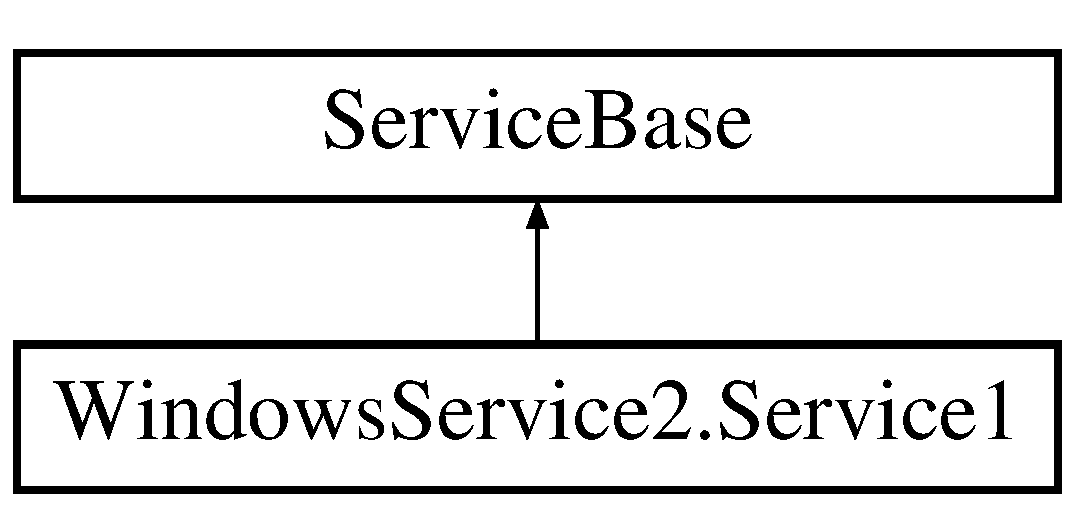
\includegraphics[height=2.000000cm]{class_windows_service2_1_1_service1}
\end{center}
\end{figure}
\subsection*{Protected Member Functions}
\begin{DoxyCompactItemize}
\item 
\mbox{\Hypertarget{class_windows_service2_1_1_service1_a7d9b5a885bc3713034b13e2e8100fd68}\label{class_windows_service2_1_1_service1_a7d9b5a885bc3713034b13e2e8100fd68}} 
override void {\bfseries On\+Start} (string\mbox{[}$\,$\mbox{]} args)
\item 
\mbox{\Hypertarget{class_windows_service2_1_1_service1_a25f5150d3c26bc7d9ea95166843de7f8}\label{class_windows_service2_1_1_service1_a25f5150d3c26bc7d9ea95166843de7f8}} 
override void {\bfseries On\+Stop} ()
\item 
override void \mbox{\hyperlink{class_windows_service2_1_1_service1_a35d81f8e347bf414b8163f34fd9d9796}{Dispose}} (bool disposing)
\begin{DoxyCompactList}\small\item\em Nettoyage des ressources utilisées. \end{DoxyCompactList}\end{DoxyCompactItemize}


\subsection{Member Function Documentation}
\mbox{\Hypertarget{class_windows_service2_1_1_service1_a35d81f8e347bf414b8163f34fd9d9796}\label{class_windows_service2_1_1_service1_a35d81f8e347bf414b8163f34fd9d9796}} 
\index{Windows\+Service2\+::\+Service1@{Windows\+Service2\+::\+Service1}!Dispose@{Dispose}}
\index{Dispose@{Dispose}!Windows\+Service2\+::\+Service1@{Windows\+Service2\+::\+Service1}}
\subsubsection{\texorpdfstring{Dispose()}{Dispose()}}
{\footnotesize\ttfamily override void Windows\+Service2.\+Service1.\+Dispose (\begin{DoxyParamCaption}\item[{bool}]{disposing }\end{DoxyParamCaption})\hspace{0.3cm}{\ttfamily [protected]}}



Nettoyage des ressources utilisées. 


\begin{DoxyParams}{Parameters}
{\em disposing} & true si les ressources managées doivent être supprimées ; sinon, false.\\
\hline
\end{DoxyParams}


The documentation for this class was generated from the following files\+:\begin{DoxyCompactItemize}
\item 
C\+:/\+Users/olymp/source/repos/\+Windows\+Service2/\+Windows\+Service2/Service1.\+cs\item 
C\+:/\+Users/olymp/source/repos/\+Windows\+Service2/\+Windows\+Service2/Service1.\+Designer.\+cs\end{DoxyCompactItemize}

%--- End generated contents ---

% Index
\backmatter
\newpage
\phantomsection
\clearemptydoublepage
\addcontentsline{toc}{chapter}{Index}
\printindex

\end{document}
